\subsection{The Localization Task}

% TODO: reference books (Siegwart and Thrun) 
During localization the main goal is to determine the coordinate transform between the local coordinate system of the robot,
and a given global frame.
For most of the problems the Global Navigation Satellite System (GNSS), like GPS provides
this information. In an ideal world the GPS data is precise and reliant, making localization algorithms unnecessary.
However, it is well known that global positioning by satellites cannot be performed in shielded environments (for example indoors),
and even outdoors, the provided precision is often not sufficient.

To overcome these deficiencies, different state estimation algorithms are used to obtain the pose of the robot in the global frame.
Localization and mapping often goes hand in hand: localization without a map
(or some kind of a representation of the environment on which the global frame is defined),
and map creation without the information about the pose is hardly possible.
If one of them is assumed to be known, the task is much easier: localization, or mapping.
If both are sought after, the Simultaneous Localization and Mapping (SLAM) problem arises,
which is significantly harder the any of them separately.
In the scope of this report, only the localization task is addressed on a given (ground truth) map.

One possible way to achieve localization is the introduction of pose hypotheses.
By this the robot's belief of its pose is a probability distribution, instead of a crisp value~\cite{Thrun2005}.
Knowing the pose exactly is not feasible in a noisy real world environment.
For a localization task, two main hardware components are used: an effector which is responsible for moving the robot,
and an exteroceptive sensor, which is responsible to obtain information about the surrounding environment (like a LiDAR, a sonar, or often a camera).
Both introduce errors and noise to the system which could be dealt with by the application of the probabilistic approach.
In the following, this modelling method is detailed.

Almost every state estimation (e.g. localization) algorithm is based on Bayesian filtering.
It servers as a foundation for these methods, and could not be implemented on its own.
A Bayes filter conducts of two main parts which are iterated over time: prediction and update (see more in \cite{Thrun2005}).
These have the following forms (respectively):
\begin{align}\label{key}
    \overline{bel}(\mathbf{x}_t) & = \int p(\mathbf{x}_t | \mathbf{x}_{t-1},\mathbf{u}_t)bel(\mathbf{x}_{t-1})\mathrm{d}\mathbf{x}_{t-1}, \\
    bel(\mathbf{x}_t)            & = \eta p(\mathbf{\mathbf{z}}_t | \mathbf{x}_t)\overline{bel}(\mathbf{x}_t),
\end{align}
where
\begin{align}\label{key}
    bel(\mathbf{x}_t)            & = p(\mathbf{x}_t|\mathbf{z}_{1:t},\mathbf{u}_{1:t}),                      \\
    \overline{bel}(\mathbf{x}_t) & = p(\mathbf{x}_t|\mathbf{z}_{1:t-1},\mathbf{u}_{1:t}) \label{eq:predbel}.
\end{align}
The notations are the following: $\mathbf{x}_t$ is the pose (position in 2D, and heading direction) at time $t$,
$\mathbf{u}_t$ is the input vector at $t$, $\eta$ is a normalization constant from  Bayes' theorem,
$\mathbf{z}_t$ is the measurement at $t$, $(.)_{1:t}$ denotes values from time $t = 1$ to $t$,
$bel(\mathbf{x}_t)$ is the belief (also called as posterior), and  $\overline{bel}(\mathbf{x}_t)$ is the predicted belief.

First, $\overline{bel}(\mathbf{x}_t)$ is calculated from the prior $bel(\mathbf{x}_{t-1})$, using the motion model (first part in the integral).
This is a prediction, because only the kinematics are incorporated, not the measurements.
Then in the update part the measurement model is considered.
This corrigates (updates) the prediction by incorporating the observations.

However, these probability distributions and integrals cannot be calculated on their own.
Each distinct filter realization addresses the solution of the Bayesian recursion differently:
the Kalman Filters use Gaussian distributions and their parametric description to estimate the pose hypotheses,
while particle filters produce a more general numerical solution by describing an arbitrary distribution via particles.
The Daum--Huang filters also use particles, but describes their movement with the help of the Fokker--Planck equation.
These realizations are explained in greater detail in Section ****.

\subsection{The Mobile Robot}
An important preliminary of localization is the introduction of the utilized hardware, the operating environment,
and their models.
In this subsection, the mobile robot itself is discussed, along with its relevant sensors,
followed by the environment representation where the robot has to be localized.

As an agent, the simulated version of ROBOTIS' TurtleBot3 is used via Robot Operating System (ROS) and Gazebo.
This two-wheeled platform is widely used for educational and prototyping purposes due to its easy handling
and well developed simulational counterpart. Although it has many useful components, here only the LiDAR and the
differential drive are discussed due to their relevancy in the localization task.
Those and the robot itself can be seen in Figure~\ref{fig:turtlebot3-burger}.
\begin{figure}[htbp]
    \centering
    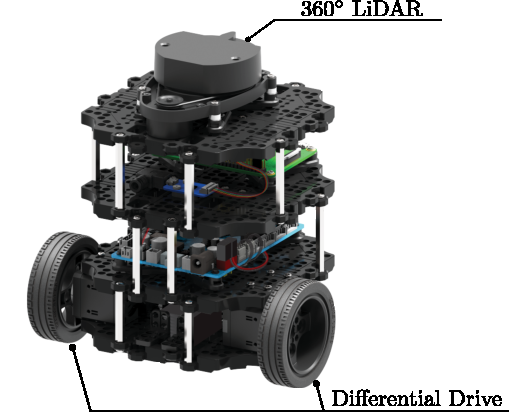
\includegraphics[width=0.5\linewidth]{turtlebot3_burger_components.pdf}
    \caption[]{ROBOTIS' TurtleBot3 Burger platform, with a mounted 360$^\circ$ LiDAR on top, and a differential drive (image source: www.robosklep.com).}
    \label{fig:turtlebot3-burger}
\end{figure}
The mounted 2D LiDAR provides range and angle measurements from the environment with $360^\circ$ field of view.
This particular model (LDS-01) has an angular resolution of $1^\circ$, detection range of $0.12-3.5$ m-s, % ! TODO validate data
and accuracy (3$\sigma$) of $\pm$15 mm-s (actually the precision is distance dependent, but this effect is not considered).
Invalid readings indicate out of range measurements. One full measurement is shown in Figure~\ref{fig:lidar-readings}.
\begin{figure}[htbp]
    \centering
    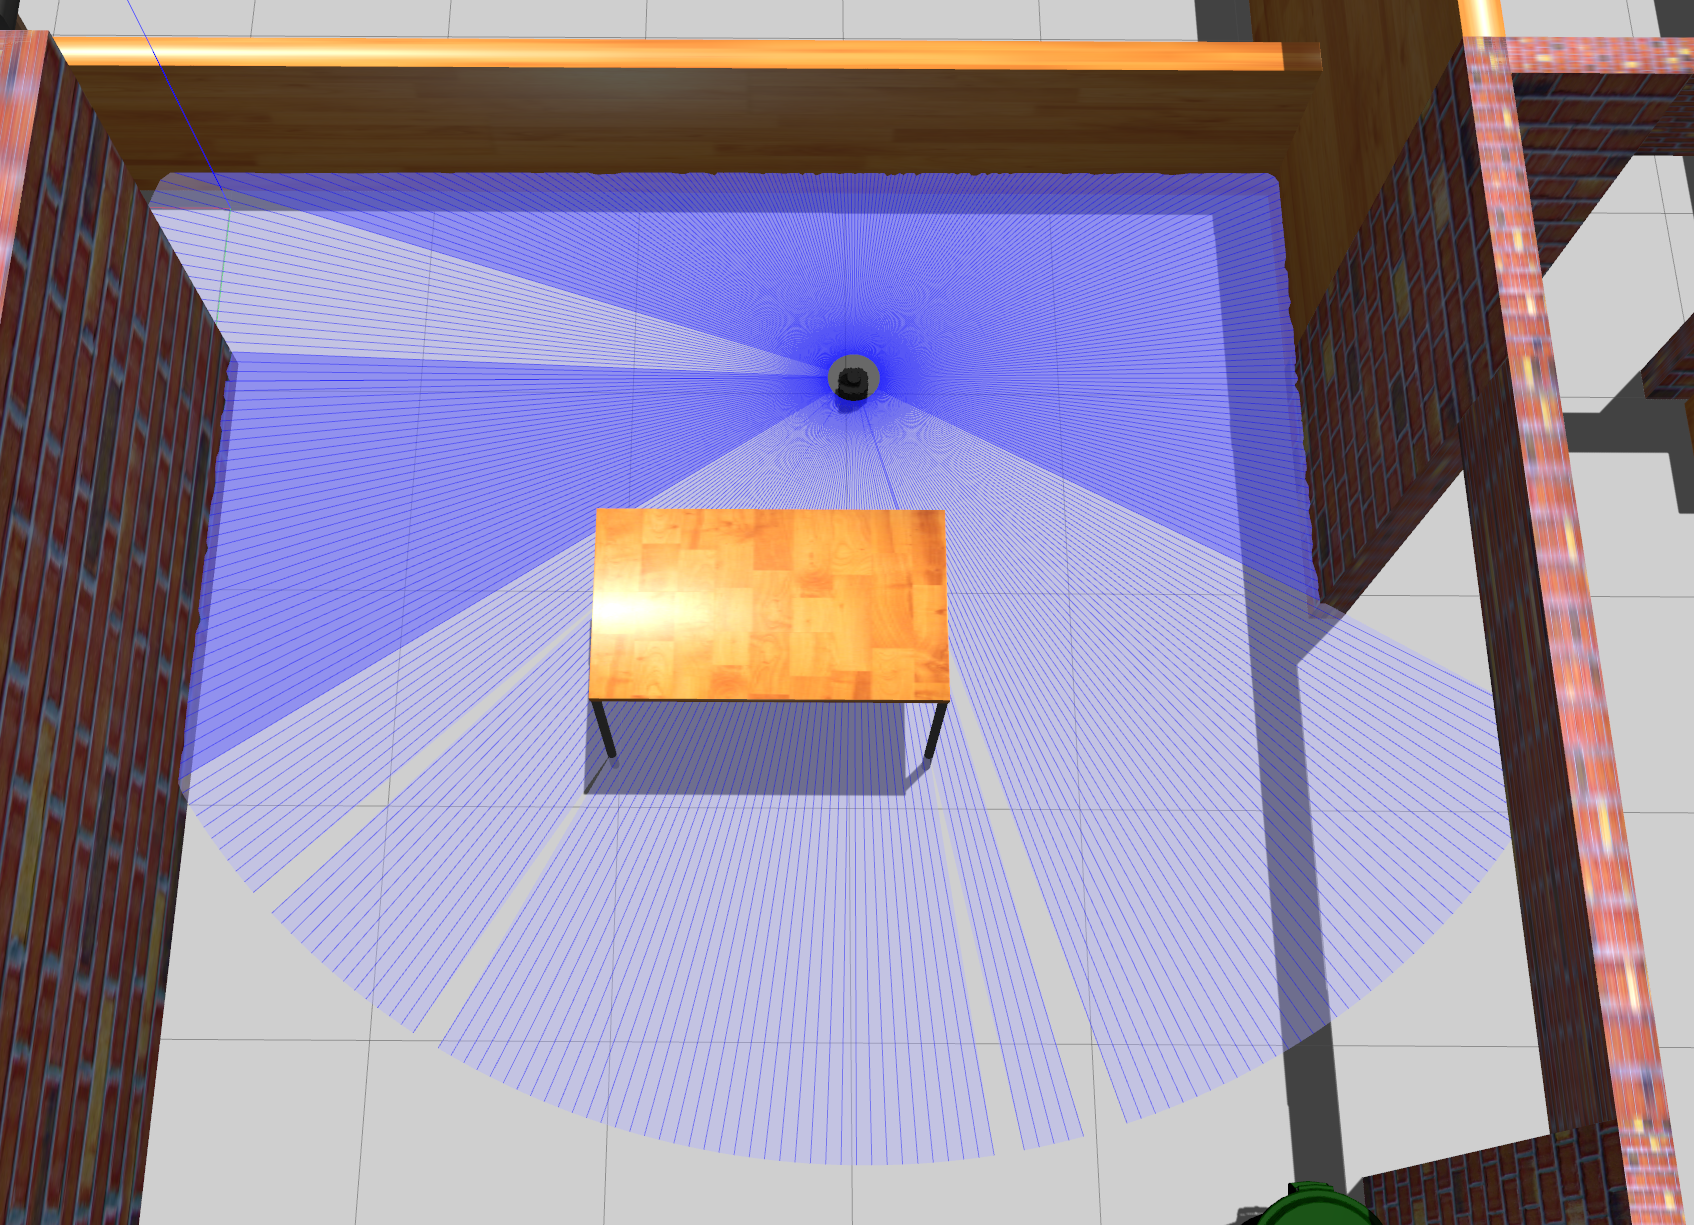
\includegraphics[width=0.6\linewidth]{lidar-visu.png}
    \caption{Visualized 2D LiDAR measurement of the TurtleBot3 in a house environment, using the Gazebo simulator.}
    \label{fig:lidar-readings}
\end{figure}

The platform has 2 independently-driven wheels, and one free turning wheel, which
makes it eligible to be modelled by differential drive kinematics.
The odometry is conducted by (simulated) rotary encoder readings from the two wheels separately.
Originally the out-of-the-box ROS-Gazebo model by ROBOTIS did not considered odometry noise,
which had to be manually added in order to efficiently model real world conditions.
Precisely modelling odometry error is a difficult task, and even nowadays is an actively researched topic \cite{Fazekas2021}.
However, this degree of precision is not required here.
Instead, both encoder readings are simply corrupted by a random variable each  ($\xi_L$ for the left wheel, $\xi_R$ for the right), obtained as
\begin{align}
    \xi_L \sim \mathcal{N}(0,\alpha v_L^{2}), \\
    \xi_R \sim \mathcal{N}(0,\alpha v_R^{2}),
\end{align}
where $\mathcal{N}(\mu,\sigma^{2})$ stands for a normal distribution with mean $\mu$ and variance $\sigma^{2}$,
$\alpha$ is a scaling parameter, and $v_L, v_R$ are the corresponding velocities. Applying this small modification,
ROS provides noisy odometry data at each tilmestep, which then can be used to establish the motion model of the robot (see Subsection~\ref{subsec:mot-model}).

\subsection{The Map}
The environment of the agent is represented by a 2D Occupancy Grid Map (OGM) \cite{Moravec1985}.
This model describes the environment by dividing it to finitely many grid cells, where each grid cell is a random binary variable,
representing that whether it’s occupied, or not.
Upon creating the OGM, the occupancy value of each cell (the probability, that its occupied) is iteratively updated.
To obtain a final map, these values are thresholded, producing values of 1 if the cell is \emph{mostly} occupied,
or 0 is its \emph{mostly not}.
The top-down view of the TurtleBot3 House by ROBOTIS and the corresponding OGM can be seen in Figure~\ref{fig:tb3-house-ogm},
which was obtained by the SLAM GMapping algorithm~\cite{Grisetti2007}.
For a pure localization task, the map is considered as ground truth,
therefore the previously introduced odometry noise was omitted during the mapping process.
\begin{figure}[htbp]
    \centering
    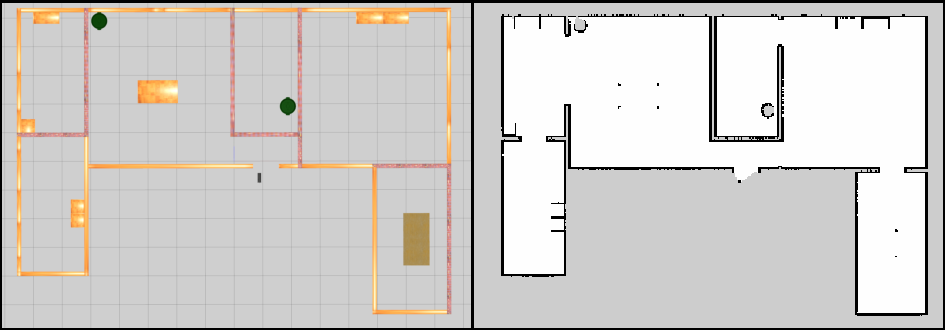
\includegraphics[width=\linewidth]{tb3-house-ogm.pdf}
    \caption{The top-down view of the TurtleBot3 House in Gazebo, and its OGM representation (mind the open doors in the building).
        Grey pixels represent unknown area, black pixels are occupied, white pixels are free cells.
        1 pixel (cell) in the OGM has a size of $0.05 \times 0.05$ m. }
    \label{fig:tb3-house-ogm}
\end{figure}
\subsection{The Motion Model}\label{subsec:mot-model}
Now that the hardware and the underlying localization task is introduced, the two main parts of the
Bayesian recursion is going to be described in the following subsections: the motion model, and the measurement model.

The motion model is used to describe the probability distribution of
$p(\mathbf{x}_t | \mathbf{x}_{t-1},\mathbf{u}_t)$. \linebreak
Without any external information, the pose of the robot at time $t$ can be estimated based on the previous pose
at time $t-1$, and the control input at time $t$. Naturally, this estimation will be disrupted by tire slippage and drift.
Due to the incremental nature, these errors are integrated over time, thus making the estimation more and more
uncertain.

The motion model describes this transition using the kinematic model of the agent.
Based on the inputs, two distinct probabilistic models can be established, introduced in \cite{Thrun2005}: the velocity motion model,
and the odometry motion model. Here, only the latter is detailed.

If the odometry of the robot is available (i.e. by integrating wheel encoder measurements),
they can be treated as a control input:
\begin{equation}
    \mathbf{u}_t = (\overline{\mathbf{x}}_t\;\;\overline{\mathbf{x}}_{t-1})^\top =
    \left(\overline{x}_t\;\;\overline{y}_t\;\;\overline{\theta}_t\;\;\overline{x}_{t-1}\;\;\overline{y}_{t-1}\;\;\overline{\theta}_{t-1}\right)^\top.
\end{equation}
The key is the fact that the relative difference between
two consecutive odometry data is a good estimation of the relative difference between
the two consecutive true poses, if the timestep is sufficiently small.

The transition between the state $\mathbf{x}_{t-1}$ and $\mathbf{x}_{t}$ is simplified as a sequence of a rotation, a translation,
and another rotation.
These are indicated in Figure~\ref{fig:odom-mot-model}. with $\delta_{\mathrm{rot1}}$, $\delta_{\mathrm{trans}}$,
and $\delta_{\mathrm{rot2}}$ respectively.
It's important to mention that this separation to rotational and translational components is arbitrary
(introduced by Thrun et al. in~\cite{Thrun2005}); for another approach, see~\cite{Eliazar2004}.
\begin{figure}[htbp]
    \centering
    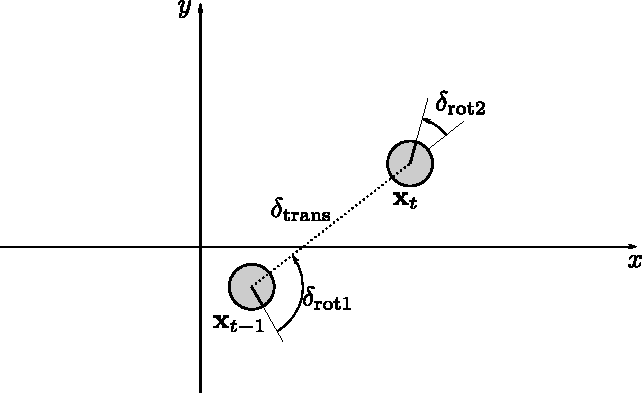
\includegraphics{odometry-motmodel.pdf}
    \caption{The rotation-translation-rotation transition sequence from state $\mathbf{x}_{t-1}$ to $\mathbf{x}_{t}$.}
    \label{fig:odom-mot-model}
\end{figure}

The control input $\mathbf{u}_t$
then transformed to the three transition components as:
\begin{align}
    \delta_{\mathrm{rot} 1} & =\arctan\!2\left(\overline{y}_{t}-\overline{y}_{t-1}, \overline{x}_{t}-\overline{x}_{t-1}\right)-\overline{\theta}_{t-1}, \\
    \delta_{\text {trans }} & =\sqrt{\left(\overline{x}_{t-1}-\overline{x}_{t}\right)^{2}+\left(\overline{y}_{t-1}-\overline{y}_{t}\right)^{2}},        \\
    \delta_{\mathrm{rot} 2} & =\overline{\theta}_{t}-\overline{\theta}_{t-1}-\delta_{\mathrm{rot} 1}.
\end{align}
To model odometry noise, the inputs are treated as random variables, formulated by
\begin{align}
    \hat{\delta}_{\mathrm{rot} 1} & = \delta_{\mathrm{rot} 1} + \xi_{\mathrm{rot1}},
    \quad                         & \xi_{\mathrm{rot1}} \sim \mathcal{N}(0,\alpha_1\delta_{\mathrm{rot1}}^2+\alpha_2\delta_{\mathrm{trans}}^2),                             \\
    \hat{\delta}_{\text {trans }} & = \delta_{\mathrm{trans}} + \xi_{\mathrm{trans}},
    \quad                         & \xi_{\mathrm{trans}} \sim \mathcal{N}(0,\alpha_3\delta_{\mathrm{trans}}^2+\alpha_4(\delta_{\mathrm{rot1}}^2+\delta_{\mathrm{rot2}}^2)), \\
    \hat{\delta}_{\mathrm{rot} 2} & = \delta_{\mathrm{rot} 2} + \xi_{\mathrm{rot2}},
    \quad                         & \xi_{\mathrm{rot2}} \sim \mathcal{N}(0,\alpha_1\delta_{\mathrm{rot2}}^2+\alpha_2\delta_{\mathrm{trans}}^2),
\end{align}
where $\alpha_1,\alpha_2,\alpha_3,\alpha_4$ are error parameters.

Then, using the control inputs and the previous state, samples from $p(\mathbf{x}_t | \mathbf{x}_{t-1},\mathbf{u}_t)$
are obtained by,
\begin{align}
    x_t          & = x_{t-1} + \hat{\delta}_{\mathrm{trans}}\cos(\theta + \hat{\delta}_{\mathrm{rot1}}), \\
    y_t          & = y_{t-1} + \hat{\delta}_{\mathrm{trans}}\sin(\theta + \hat{\delta}_{\mathrm{rot1}}), \\
    \theta_t     & = \theta_{t-1} + \hat{\delta}_{\mathrm{rot1}} + \hat{\delta}_{\mathrm{rot2}},         \\
    \mathbf{x}_t & = \left(x_t\;\;y_t\;\;\theta_t\right)^\top.
\end{align}


